\documentclass[10pt,border=4pt]{standalone}
% 2026-09-28 (review pass E: V17-08): set in Charter (mathdesign), the paper's body and figure font, at 10pt, instead
% of 12pt Latin Modern; wider row/column spacing gives a natural width of about 270pt, close to the \columnwidth
% (0.65\textwidth, about 277pt) at which main.tex includes it, so the labels come out near 10pt instead of 13.4pt.
\usepackage[T1]{fontenc}\usepackage{amsmath}\usepackage[bitstream-charter]{mathdesign}
\usepackage{tikz}\usepackage{quantikz}
\usetikzlibrary{arrows.meta,positioning,fit,calc}

% palette harmonised with Paper 2 (fig_circuit_native)
\definecolor{inkPrim}{HTML}{1B1B1B}\definecolor{inkMute}{HTML}{6E6E6E}
\definecolor{coral}{HTML}{D55E00}\definecolor{blue}{HTML}{0072B2}
\definecolor{teal}{HTML}{1E7A6E}\definecolor{ox}{HTML}{B5651D}

\begin{document}
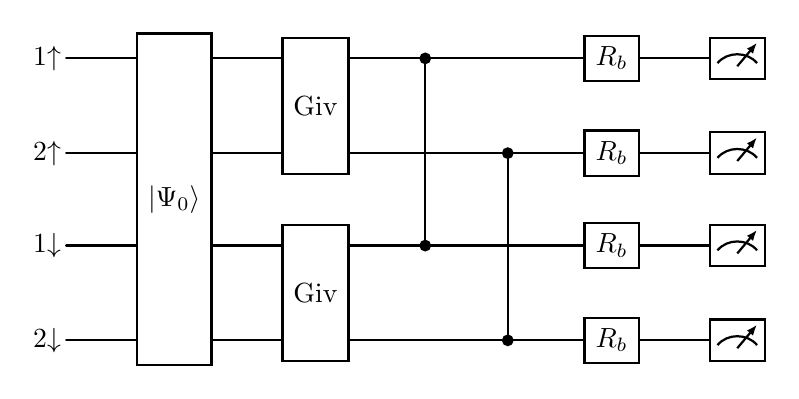
\begin{tikzpicture}[font=\rmfamily]
\node[inner sep=1pt] (circ) at (0,0) {%
\begin{quantikz}[row sep=0.6cm,column sep=0.9cm]
  \lstick{$1{\uparrow}$} & \gate[4]{\lvert\Psi_0\rangle} & \gate[2]{\text{Giv}} & \ctrl{2} &            & \gate{R_b} & \meter{} \\
  \lstick{$2{\uparrow}$} & & &            & \ctrl{2}   & \gate{R_b} & \meter{} \\
  \lstick{$1{\downarrow}$} & & \gate[2]{\text{Giv}} & \control{} &          & \gate{R_b} & \meter{} \\
  \lstick{$2{\downarrow}$} & & &            & \control{} & \gate{R_b} & \meter{}
\end{quantikz}};
\end{tikzpicture}
\end{document}
